\question[3]
Schreibe eine Funktion \texttt{baum}, die den abgebildeten Baum zurückgibt.
Nutze dazu unsere Baum-Klasse.
Verschachtele die Baum-Aufrufe aus Lesbarkeitsgründen
höchstens einmal und gib den temporären Teilbäumen sprechende Namen.

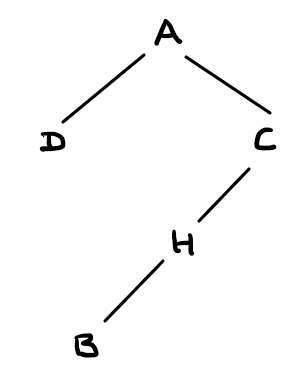
\includegraphics[height=4cm]{\pfad/Baum/Aufgaben/baumdef_02/baumdef_02.png}

\begin{solutionbox}{5cm}
\begin{lstlisting}
def baum():
    h = Baum('H',Baum('B'),None)
    c = Baum('C',h,None)
    a = Baum('A',Baum('D'),c)
    return a
\end{lstlisting}
\end{solutionbox}
